\documentclass{article}
\usepackage[utf8]{inputenc}
\usepackage[spanish]{babel}
\usepackage{listings}
\usepackage{amsmath}
\usepackage{graphics, graphicx}
\usepackage[colorlinks]{hyperref}

\lstset{frame=tb,
  language=Bash,
  aboveskip=3mm,
  belowskip=3mm,
  showstringspaces=false,
  columns=flexible,
  basicstyle={\small\ttfamily},
  numbers=none,
  numberstyle=\tiny\color{gray},
  keywordstyle=\color{blue},
  commentstyle=\color{dkgreen},
  stringstyle=\color{mauve},
  breaklines=true,
  breakatwhitespace=true,
  tabsize=3
}

\begin{document}
\begin{titlepage}
  \centering
  
\includegraphics[width=0.5\textwidth]{images/logo-ugr.png}\par
  \vspace{1cm}
  {\Large\scshape Gestión de Información en la Web \par}
  {\huge\bfseries Desarrollo de un Sistema de Recomendación basado en filtrado
  colaborativo \par}
  \vspace{0.2cm}
  {\scshape Práctica 4 \par}
  \vfill
  {\large Víctor Vázquez Rodríguez  \par}
  {victorvazrod@correo.ugr.es \par}
  {76664636R \par}
  \vfill
  {\large Máster universitario en Ingeniería Informática \par}
  \vspace{0.2cm}
  {Curso 2019/20 \par}
\end{titlepage}

\tableofcontents\newpage

\section{Introducción}

Hoy en día, el procesamiento de lenguaje natural (NLP por sus siglas en inglés)
es uno de los principales campos de estudio en inteligencia artificial y
\textit{deep learning}. Este campo se centra en la interpretación del lenguaje
humano por parte de ordenadores, permitiendo cosas como el control de
dispositivos con la voz o el análisis y traducción de textos.

Un aspecto muy importante a la hora de procesar y analizar lenguaje natural es
la representación que usamos del mismo, concretamente, cómo representamos las
palabras de forma que un ordenador pueda trabajar con ellas de forma eficiente y
obtener información relevante de su significado y su contexto. Desde el punto de
vista del \textit{machine learning}, podríamos interpretar las palabras de un
texto (o de cualquier conjunto de palabras) como valores de una variable
categórica, donde cada palabra distinta supone una categoría. Uno de los métodos
más comunes y usados para representar este tipo de variables es la codificación
\textit{one-hot}, que nos permite obtener un vector de valores númericos para
cada categoría.

No obstante, esta técnica presenta grandes limitaciones para el procesamiento de
lenguaje natural, de forma que surgen los \textit{word embeddings}. Se trata de
modelos apoyados en las redes neuronales para la proyección o incrustación
(traducción literal de \textit{embedding}) de palabras en un espacio
vectorial~\cite{definition}. En la sección \ref{sec:one-hot-limitations} de este
documento se explican las limitaciones de la codificación \textit{one-hot} y
por qué son necesarios los \textit{word embeddings}, mientras que en la sección
\ref{sec:techniques} se exponen algunas de las técnicas más utilizadas. Al
final, en la sección \ref{sec:example}, se muestra un ejemplo práctico de NLP
con \textit{word embeddings}.
\newpage
\section{Algoritmo}

El objetivo de un sistema de recomendación es presentar a un usuario elementos que no ha visto/consumido y que pueden ser de su interés. Una manera de conseguir esto es mediante las llamadas técnicas de filtrado colaborativo, las cuáles se basan en las acciones de los usuarios (dar "me gusta"/"no me gusta", puntuar del 1 al 5, ...) para obtener las recomendaciones, aplicando modelos como KNN (\textit{K Nearest Neighbors}, que es el que usaremos en esta práctica.

La idea principal de KNN es buscar los $k$ elementos o vecinos más similares a uno dado y, a partir de ellos, obtener las recomendaciones. Estos elementos pueden ser ítems (basado en ítems) o usuarios del sistema (basado en usuarios). Nosotros aplicaremos KNN basado en usuarios para nuestro sistema de recomendación, de forma que buscamos los usuarios más parecidos al usuario activo para recomendarle las películas que les han gustado a estos otros usuarios.

Las películas son valoradas del 1 al 5, por lo que tenemos que tener en cuenta, además, que distintos usuarios valoran un ítem que les ha gustado de forma diferente, por lo que, lo primero que hacemos, es calcular un valor para equilibrar esos desajustes de escala e interpretación. La fórmula para realizar este cálculo se muestra a continuación, donde $S_u$ es el conjunto de ítems valorados por el usuario $u$ y $n_{S_u}$ es el número de ítems del mismo.

\begin{equation}
    \bar{r}(u) = \frac{\sum_{i \epsilon S_u} r(u, i)}{n_{S_u}}
\end{equation}

Una vez obtenido este valor para los usuarios, podemos calcular la similitud entre un usuario $u$ y otro usuario $v$ con la ecuación (2), donde $r(u,i)$ es la valoración dada por el usuario $u$ para el ítem $i$.

\begin{equation}
    sim(u,v) = \frac{\sum_{i \epsilon S_{uv}}(r(u,i) - \bar{r}(u))(r(v,i) - \bar{r}(v))}{\sqrt{\sum_{i \epsilon S_{uv}}(r(u,i) - \bar{r}(u))^2} \sqrt{\sum_{i \epsilon S_{uv}}(r(v,i) - \bar{r}(v))^2}}
\end{equation}

Usando esta ecuación, obtenemos la similitud con el usuario activo para todos los demás usuarios presentes en la base de datos, quedándonos con los $k$ usuarios con mayor similitud. Un problema con el que nos podemos encontrar es que, si un usuario sólo tiene un ítem en común con el usuario activo, pero con idéntica valoración, la función de similitud devolverá 1, con lo que podría entrar este usuario en el vecindario. Esto no es realista, ya que solo tienen una película en común y eso no nos ayuda a la hora de obtener recomendaciones adecuadas. Para evitar esto, solo calculamos la similitud de los usuarios que tengan, al menos, 5 películas en común con el usuario activo.

Una vez tenemos definido el vecindario, buscamos los ítems a recomendar al usuario activo entre los que han sido valorados por sus vecinos y no por él. Para obtener estas recomendaciones, estimamos la valoración que le daría a cada ítem el usuario activo $u$ usando la siguiente ecuación:

\begin{equation}
    \hat{r}(u,i) = \bar{r}(u) + C\sum_v sim(u,v)(r(v,i) - \bar{r}(v))
\end{equation}

Donde la constante $C$ se calcula de la siguiente manera:

\begin{equation}
    C = \frac{1}{\sum_v |sim(u,v)|}
\end{equation}

Cuando ya tenemos la valoración estimada de todos los ítems, seleccionamos solo los de valoración más alta (4 o 5), que son las recomendaciones que le mostramos al usuario activo. No obstante, nos hemos encontrado con que, al sumar el valor $\bar{r}(u)$ en la fórmula de estimación de la valoración, obtenemos valores mayores de 5 para la misma. Para solucionar esto, lo que hacemos es reescalar todo el conjunto de valoraciones estimadas para que estén dentro del intervalo $[1, 5]$ usando la siguiente fórmula, donde $x$ es la valoración estimada a reescalar y $max$ es la valoración máxima que se ha obtenido.

\begin{equation}
    \frac{x-1}{max-1}4+1
\end{equation}\newpage
\section{Interfaz}

En esta sección, vamos a mostrar la interfaz de usuario de la aplicación web que se ha desarrollado para servir como \textit{frontend} al sistema de recomendación. Al acceder a la web, el usuario es recibido con un mensaje de bienvenida que le explica sencillamente en qué consiste el sistema.
\\\\
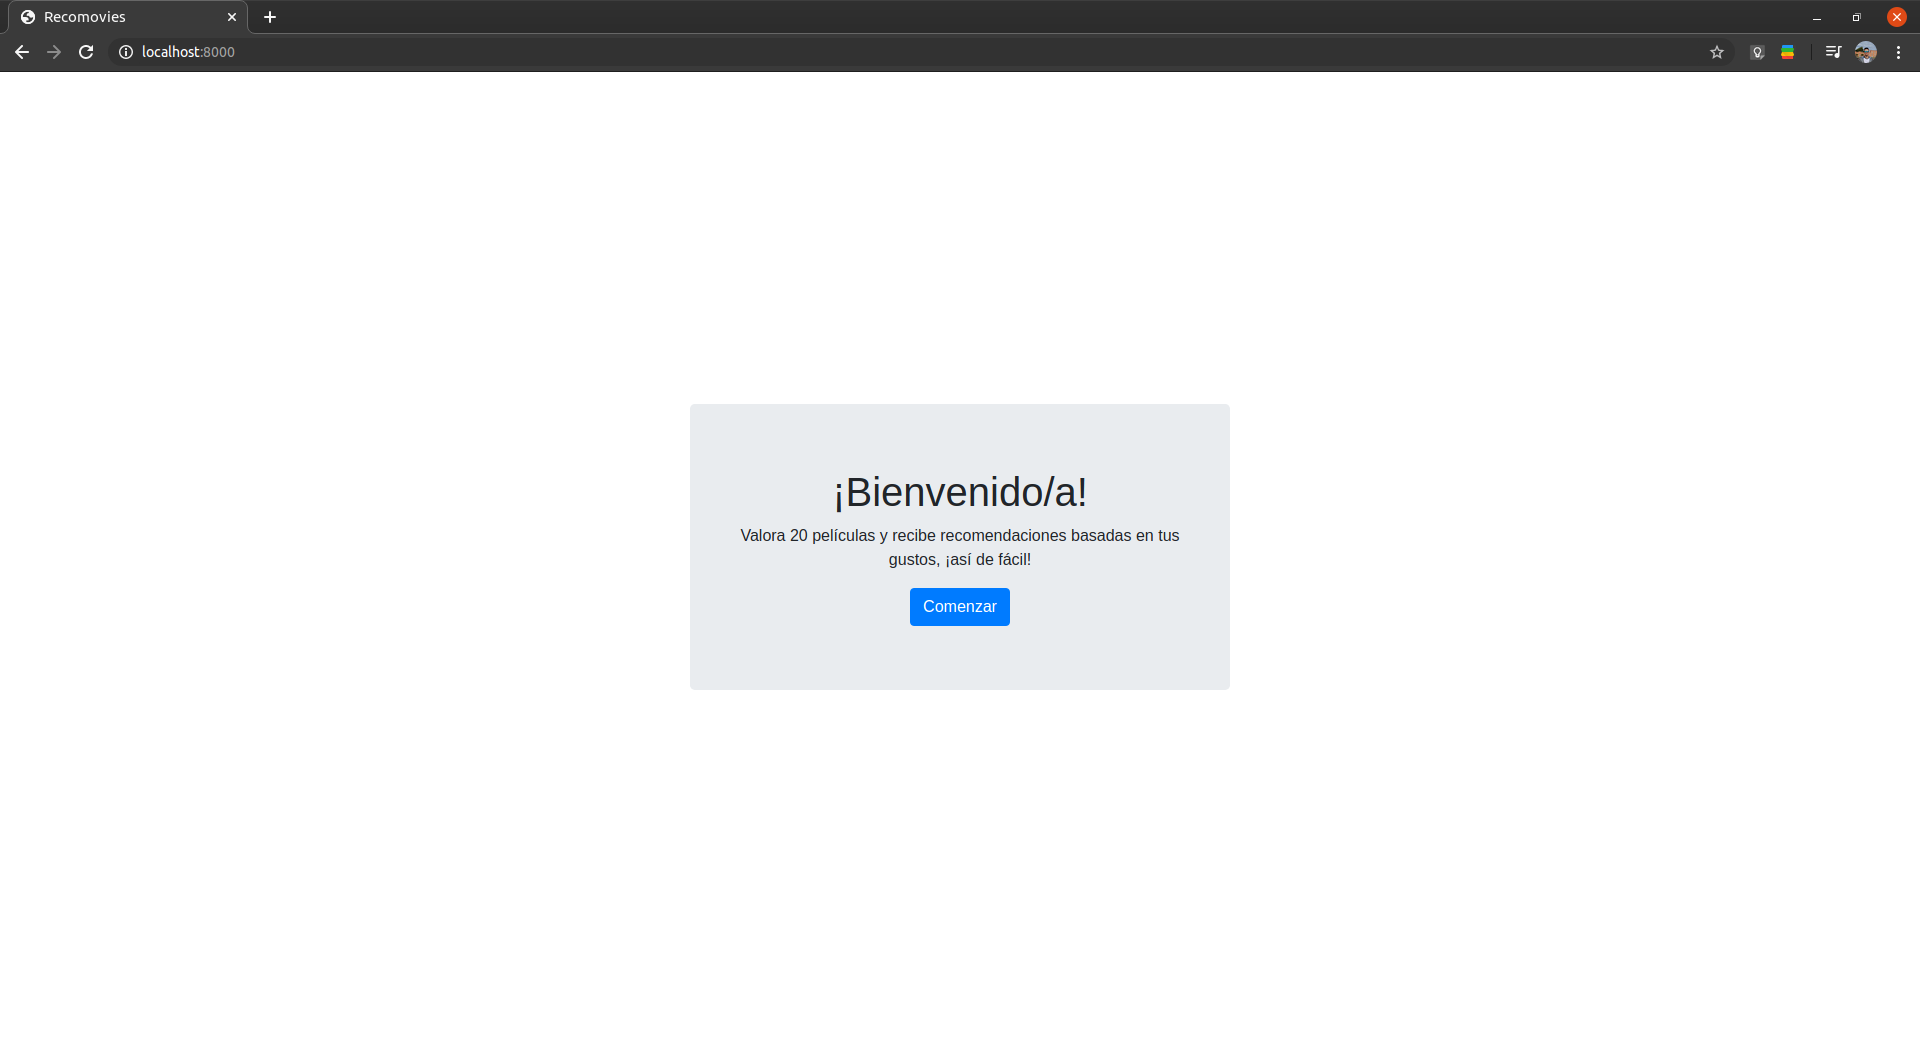
\includegraphics[width=\textwidth,height=\textheight,keepaspectratio]{images/index.png}
\\\\
Cuando el usuario pulsa en el botón de "Comenzar", se crea una nueva sesión para él y se obtienen de forma aleatoria las 20 películas que debe valorar. Estas películas se le muestran de forma secuencial al usuario en pantallas como la que se puede ver a continuación:
\\\\
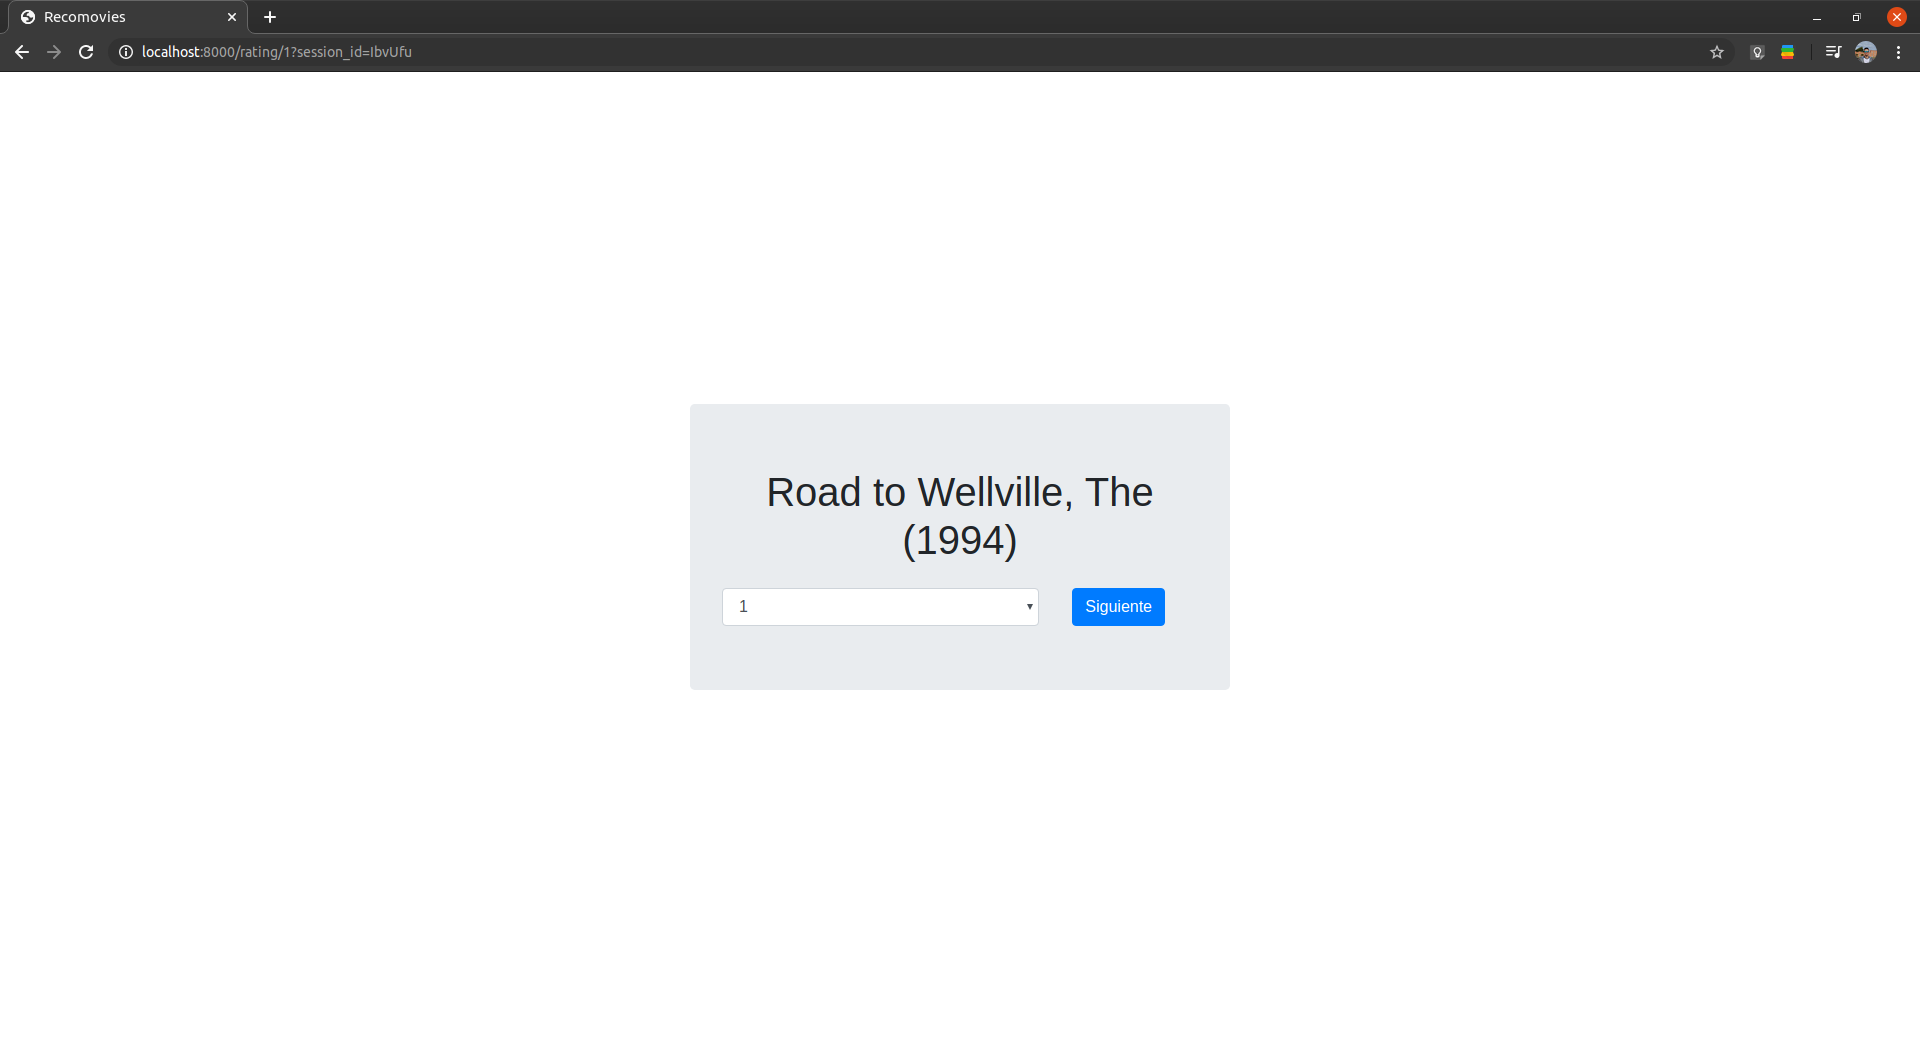
\includegraphics[width=\textwidth,height=\textheight,keepaspectratio]{images/rating.png}
\\\\
Una vez se han valorado las 20 películas, el sistema calcula el vecindario y obtiene las recomendaciones, mostrándoselas al usuario en la pantalla de resultados.
\\\\
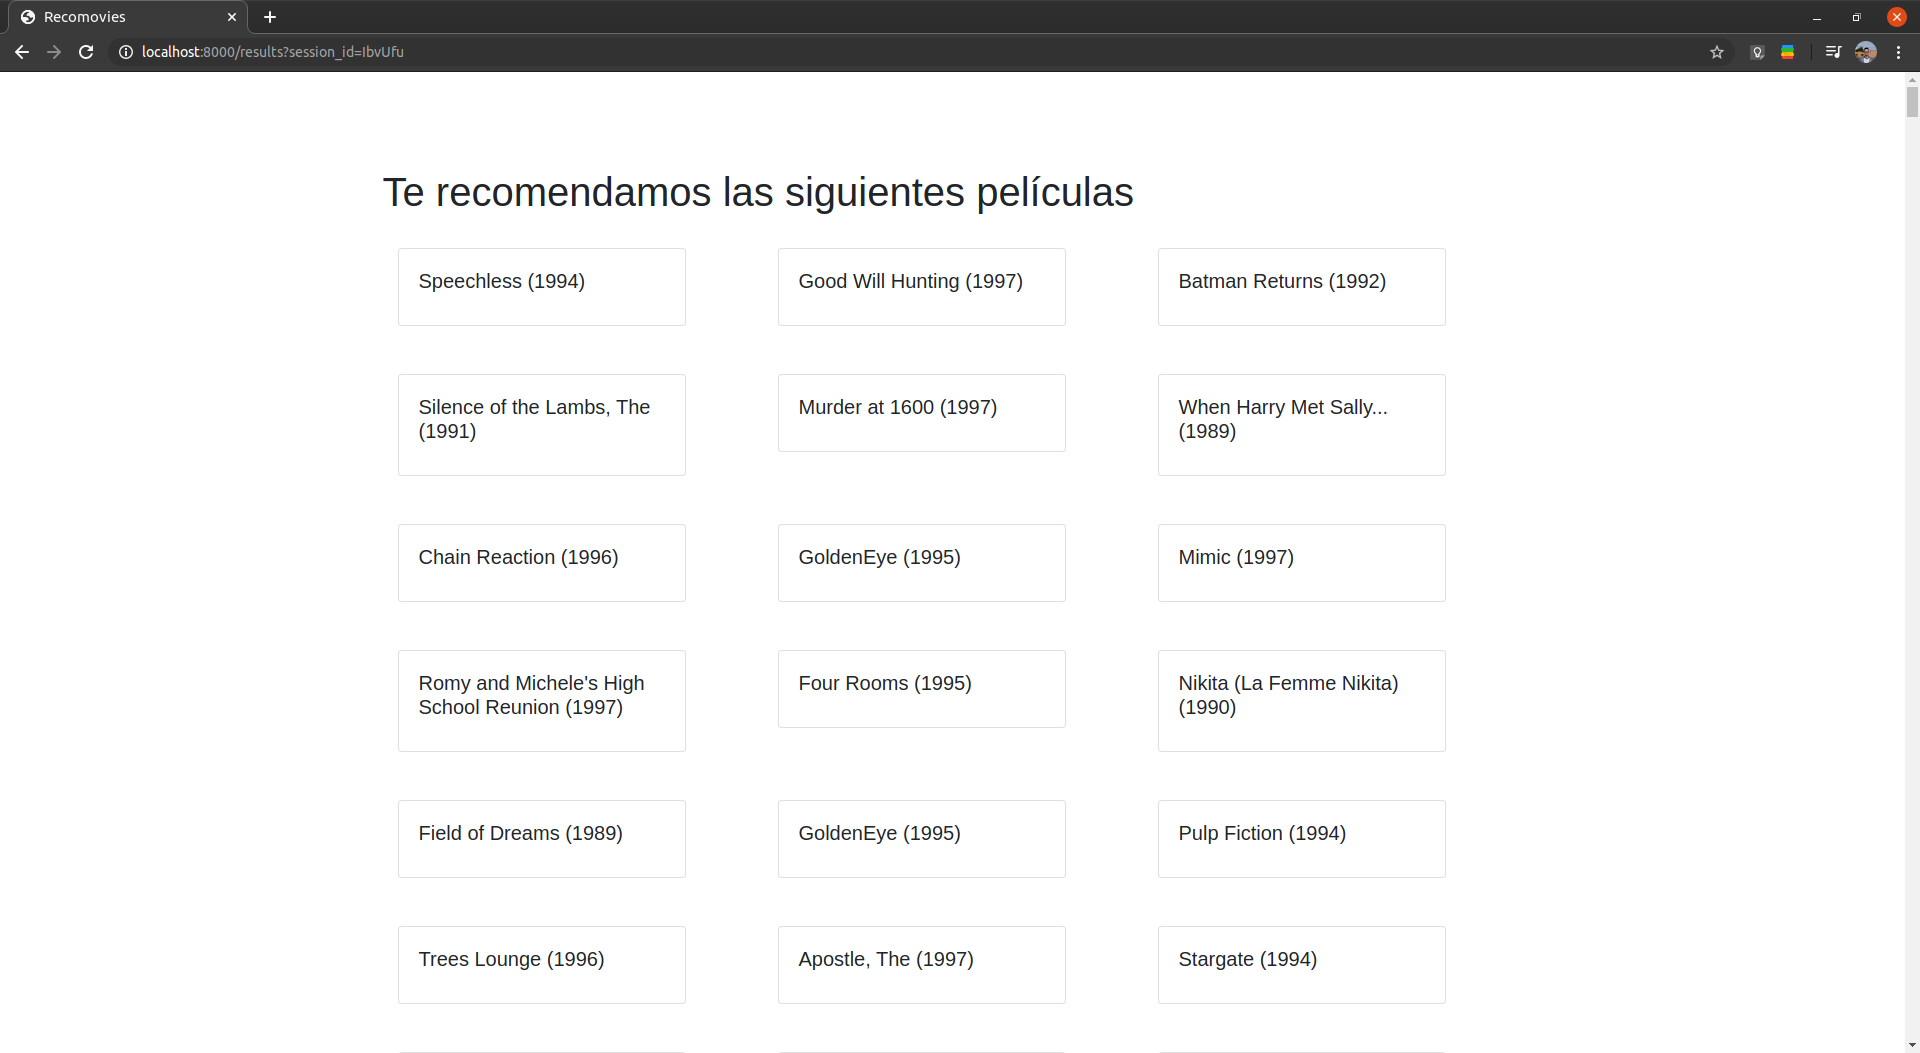
\includegraphics[width=\textwidth,height=\textheight,keepaspectratio]{images/results.png}

\subsection{Manual de uso}

Para ejecutar la aplicación, debe tener una carpeta \textit{data} en la raíz del proyecto que contenga los ficheros \textit{u.data} y \textit{u.item} con los datos. La aplicación leerá estos datos y los cargará en una base de datos SQLite también en la raíz.

Debe tener instaladas en sus sistema las herramientas de Go, con lo que podría lanzar la aplicación con el siguiente comando:

\begin{lstlisting}
go run main.go
\end{lstlisting}

En la terminal se le mostrará el progreso de carga de datos e inicialización del servidor web, tras lo cuál, debería poder acceder a la aplicación con su navegador web a través de la dirección \textit{http://localhost:8000}.\newpage
\section{Referencias}

Para la realización de esta práctica se han usado algunas fuentes complementarias al guión proporcionado, las cuáles se indican a continuación:

\begin{itemize}
    \item \href{https://golang.org/doc/}{Documentación de Go}, usada para consultar dudas sobre ordenación de \textit{arrays}.
    \item \href{https://gin-gonic.com/docs/}{Documentación de Gin}, \textit{framework} usado para el desarrollo de la aplicación web.
    \item \href{https://gorm.io/docs/}{Documentación de GORM}, usada para consultar cómo se componían las consultas a la base de datos.
\end{itemize}\newpage
\end{document}
